\documentclass[11pt,letterpaper,titlepage]{article}

\usepackage{geometry}
\geometry{left=2cm,right=2cm,top=2cm,bottom=3cm}

\usepackage{setspace}
\onehalfspacing

\usepackage{booktabs}

\usepackage{fancyhdr}

\pagestyle{fancy}
\lhead{}
\rhead{}
\lfoot{ECEN 749 Section 601 Assignment 1}
\cfoot{\thepage}
\rfoot{@Lei Wang (Wilson)}
\renewcommand{\headrulewidth}{0pt}
\renewcommand{\headwidth}{\textwidth}
\renewcommand{\footrulewidth}{0.4pt}
\newcommand{\RomanNumeralCaps}[1]
{\MakeUppercase{\romannumeral #1}}
    
\usepackage{xcolor}
\definecolor{vgreen}{RGB}{104,180,104}
\definecolor{vblue}{RGB}{49,49,255}
\definecolor{vorange}{RGB}{255,143,102}

\usepackage{listings}

\lstdefinestyle{verilog-style}
{
    language=Verilog,
    basicstyle=\small\ttfamily,
    keywordstyle=\color{vblue},
    identifierstyle=\color{black},
    commentstyle=\color{vgreen},
    % numbers=left,
    numberstyle=\tiny\color{black},
    numbersep=11pt,
    tabsize=4,
    moredelim=*[s][\colorIndex]{[}{]},
    literate=*{:}{:}1
}    

\usepackage{tikz}

\usetikzlibrary{automata, positioning, arrows}

\newcounter{wavenum}

\setlength{\unitlength}{0.1cm}
% advance clock one cycle, not to be called directly
\newcommand*{\clki}{
  \draw (t_cur) -- ++(0,.3) -- ++(.5,0) -- ++(0,-.6) -- ++(.5,0) -- ++(0,.3)
    node[time] (t_cur) {};
}

\newcommand*{\bitvector}[3]{
  \draw[fill=#3] (t_cur) -- ++( .1, .3) -- ++(#2-.2,0) -- ++(.1, -.3)
                         -- ++(-.1,-.3) -- ++(.2-#2,0) -- cycle;
  \path (t_cur) -- node[anchor=mid] {#1} ++(#2,0) node[time] (t_cur) {};
}

% \known{val}{length}
\newcommand*{\known}[2]{
    \bitvector{#1}{#2}{white}
}

% \unknown{length}
\newcommand*{\unknown}[2][XXX]{
    \bitvector{#1}{#2}{black!20}
}

% \bit{1 or 0}{length}
\newcommand*{\bit}[2]{
  \draw (t_cur) -- ++(0,0.6*#1) -- ++(#2,0) %-- ++(0,-0.6*#1)
    node[time] (t_cur) {};
}

% \unknownbit{length}
\newcommand*{\unknownbit}[1]{
  \draw[ultra thick,black!50] (t_cur) -- ++(#1,0) node[time] (t_cur) {};
}

% \nextwave{name}
\newcommand{\nextwave}[1]{
  \path (0,\value{wavenum}) node[left] {#1} node[time] (t_cur) {};
  \addtocounter{wavenum}{-1}
}

% \clk{name}{period}
\newcommand{\clk}[2]{
    \nextwave{#1}
    \FPeval{\res}{(\wavewidth+1)/#2}
    \FPeval{\reshalf}{#2/2}
    \foreach \t in {1,2,...,\res}{
        \bit{\reshalf}{1}
        \bit{\reshalf}{0}
    }
}

% \begin{wave}[clkname]{num_waves}{clock_cycles}
\newenvironment{wave}[3][time]{
  \begin{tikzpicture}[draw=black, yscale=.7,xscale=1]
    \tikzstyle{time}=[coordinate]
    \setlength{\unitlength}{0.5cm}
    \def\wavewidth{#3}
    \setcounter{wavenum}{0}
    \nextwave{#1}
    \foreach \t in {0,1,...,\wavewidth}{
      \draw[dotted] (t_cur) +(0,.5) node[above] {\t 0} -- ++(0,.4-#2);
      \clki
    }
}{\end{tikzpicture}}

\begin{document}

\begin{enumerate}
    \item %Q1
    
    \begin{enumerate}
        \item %Q1a
        
        The timing waveform is shown as the following: 
        
        \begin{figure}[ht]
            \centering
                \begin{wave}{9}{15}[h!]
                    \nextwave{A} \bit{0}{0} \bit{1}{15}
                    \nextwave{B} \bit{1}{0} \bit{0}{15}
                    \nextwave{C} \bit{0}{0} \bit{1}{15}
                    \nextwave{D} \bit{0}{0} \bit{1}{15}
                    \nextwave{X} \unknown{1} \bit{0}{14}
                    \nextwave{Y} \unknown{4} \bit{0}{11}
                    \nextwave{Z} \unknown{5} \bit{1}{10}
                    \nextwave{E} \unknown{1} \bit{0}{7} \bit{1}{7}
                    \nextwave{F} \unknown{5} \bit{0}{10}
            \end{wave}
            \caption{Timing waveform for Q1)a).}
            \label{fig:my_label}
        \end{figure}
        
        \item %Q1b
        
        \lstinputlisting[style={verilog-style}]{1b.txt}
        
        \item %Q1c
        
        \lstinputlisting[style={verilog-style}]{1c.txt}
        
        \item %Q1D
        
        \lstinputlisting[style={verilog-style}]{1d.txt}
        
    \end{enumerate}
    
    \newpage
    
    \item %Q2
    
    The transition table is listed as the following:
    
    \begin{table}[ht]
    \centering
    \begin{tabular}{@{}cccccc@{}}
    \toprule
    State & x & Clk        & Rst & z & Next state \\ \midrule
    A     & 1 & $\uparrow$ & 0   & 0 & A          \\ \midrule
    A     & 0 & $\uparrow$ & 0   & 0 & B          \\ \midrule
    B     & 0 & $\uparrow$ & 0   & 1 & A          \\ \midrule
    B     & 1 & $\uparrow$ & 0   & 0 & C          \\ \midrule
    C     & 0 & $\uparrow$ & 0   & 1 & D          \\ \midrule
    C     & 1 & $\uparrow$ & 0   & 1 & D          \\ \midrule
    D     & 0 & $\uparrow$ & 0   & 0 & A          \\ \midrule
    D     & 1 & $\uparrow$ & 0   & 0 & B          \\ \midrule
    X     & X & $\uparrow$ & 1   & X & A          \\ \bottomrule
    \end{tabular}
    \caption{Transition table for question 2. X represents all possible states or numbers.}
    \end{table}
    
    The corresponding state transition diagram is hence:
    
    \begin{figure}[ht]
        \centering
        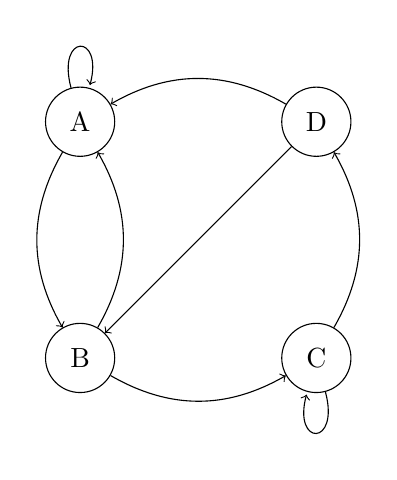
\begin{tikzpicture}
            \node[state] (A) {A};
            \node[state, below of=A, yshift=-2cm] (B) {B};
            \node[state, right of=B, xshift=2cm] (C) {C};
            \node[state, above of=C, yshift=2cm] (D) {D};
            \draw (A) edge[loop above] node{} (A);
            \draw [->] (A) edge[bend right] node{} (B);
            \draw [->] (B) edge[bend right] node{} (A);
            \draw [->] (B) edge[bend right] node{} (C);
            \draw (C) edge[loop below] node{} (C);
            \draw [->] (C) edge[bend right] node{} (D);
            \draw [->] (D) edge[bend right] node{} (A);
            \draw [->] (D) edge[] node{} (B);
        \end{tikzpicture}
        \caption{Mealy state transition diagram for question 2.}
    \end{figure}
    
    \item %Q3
    
    % write the pseudo-code first
    % then implement the Verilog code
    % maybe use different approach, i.e. the behaviour model and the structural model to write the code
    % do a final check after done with the questions
    % do a final-final check before submitting the questions
\end{enumerate}

\end{document}
